%************************************************
\chapter{Background material and Supporting Technologies}
\label{ch:background}
%******The \cite{zhang_studies_2000} paper studies and explains very well the capacity fade refers to the gradual decline in a lithium-ion battery's ability to store energy, showing as reduced device runtime or diminished electric vehicle driving range. This phenomenon is driven by several key mechanisms:*****************************************

This chapter shows the basic background material and supporting tools that were used in the project. The first section covers the main ideas for battery health monitoring, including explanations of key battery parameters such as State of Charge (SoC), State of Health (SoH), and Remaining Useful Life (RUL). Also, the work covers the basic evaluation metrics used to check model performance and provides a discussion of battery wear mechanisms that directly affect health estimation accuracy. The chapter also looks at the technical challenges in battery health monitoring, from the complexity of chemical processes to the difficulties of real-world use. The second section shows the software tools and platforms that helped the research and development process, from parameter tuning and experiment tracking to data display and version control.

\section{Core Concepts}

This section covers the main ideas basic to battery health monitoring, including detailed explanations of key battery parameters, evaluation metrics, wear mechanisms, and technical challenges. Battery technology serves as the foundation for energy storage systems across many applications. Modern batteries mainly fall into several types, including lithium-ion, lead-acid, nickel-metal hydride, and flow batteries, each with different chemical properties, energy densities, and lifecycle characteristics. The health of these batteries is shown by parameters such as state of charge (SoC), state of health (SoH), capacity fade, internal resistance, and wear rates, which together determine performance and longevity. Monitoring these parameters presents unique challenges due to the complex, nonlinear relationships between observable measurements and battery conditions. Artificial intelligence and machine learning approaches offer good solutions to these challenges by enabling pattern recognition across multidimensional battery data. Deep learning architectures, particularly recurrent neural networks and transformers, have shown exceptional ability in extracting temporal patterns from battery operational data, making them especially valuable for health prediction in dynamic usage scenarios. 

%Battery fundamentals (types, chemistry, operating principles)
%Key health monitoring parameters for batteries
%AI/ML fundamentals relevant to your application

\textbf{Time Series and Spectral Analysis of Battery Data}

Time series analysis studies how battery parameters like voltage, current, and SoC change over time. It helps model and predict battery behavior, find trends, and detect problems in the time domain. Time series analysis breaks down battery data into three basic parts that show different patterns in battery behavior and wear.

\textbf{Trend Component} shows the long-term direction of battery parameters over time, capturing how the battery wears down and reflects basic changes in battery chemistry and structure. In battery health monitoring, trend analysis shows capacity loss patterns, where SoH slowly decreases over hundreds or thousands of charge-discharge cycles due to the wear mechanisms detailed in Section~\ref{sec:degradation}. The trend component is useful for RUL prediction, as it shows the rate of wear and helps set expected levels for battery performance decline under specific use conditions.

\textbf{Seasonal/Cyclic Component} finds repeated patterns that happen at regular times in battery data, showing periodic effects like daily use cycles, temperature changes, or charging schedules. In car applications, seasonal patterns may show as daily driving patterns that affect SoC changes, while in fixed energy storage systems, seasonal parts often match daily energy demand cycles or seasonal temperature changes that affect battery efficiency and capacity. These cyclic patterns are important for understanding how outside factors affect battery behavior and for building models that can handle predictable changes in performance.

\textbf{Irregular/Noise Component} includes random changes and unpredictable variations that cannot be linked to trend or seasonal patterns, including measurement noise, sudden load changes, and random environmental factors. In battery monitoring systems, irregular parts may come from sensor limits, electrical interference, sudden acceleration events in vehicles, or unexpected temperature spikes. While these parts represent uncertainty in the data, proper analysis of noise patterns is important for building strong estimation methods that can tell the difference between real battery state changes and measurement errors.

Along with this time-based approach, spectral analysis is a frequency-domain method that studies the dynamic behavior of battery systems by breaking down time-series data into its frequency parts, showing periodic patterns, noise characteristics, or system responses that may not be clear in the time domain. 

\textbf{Fast Fourier Transform (FFT) in Battery Analysis}

The Fast Fourier Transform (FFT) is a key computational tool for spectral analysis that efficiently converts time-domain battery data into frequency-domain representations. FFT analysis is particularly valuable for battery health monitoring because it can identify hidden periodic patterns in battery operational data that are not obvious when looking at the raw time series.

In battery applications, FFT helps identify several important patterns:

\begin{itemize}
\item \textbf{Charge-discharge cycle frequencies}: Regular charging and discharging patterns create dominant frequencies that FFT can detect, helping to understand battery usage patterns and predict future behavior.
\item \textbf{Daily and seasonal usage patterns}: FFT can identify daily usage cycles (24-hour periods) and longer seasonal patterns that affect battery performance in real-world applications.
\item \textbf{High-frequency noise and electrical interference}: FFT analysis can separate measurement noise from actual battery signals, improving data quality for health estimation models.
\item \textbf{Aging-related frequency changes}: As batteries wear down, the frequency characteristics of their operational patterns may shift, providing early indicators of health decline.
\end{itemize}


The FFT analysis becomes particularly important when using advanced machine learning models like TimesNet (discussed in Section~\ref{sec:timesnet_model}), which automatically discovers multiple periodic patterns in battery data using FFT-based period detection. By identifying the strongest frequency components in battery operational data, FFT enables the model to focus on the most relevant periodic behaviors for accurate health prediction.

\textbf{Cascade spectrum analysis} can be combined with traditional spectral methods to provide multi-level frequency domain breakdown. This cascaded approach is useful for battery applications where wear mechanisms work at multiple frequency ranges, from high-frequency electrical impedance changes to low-frequency capacity fade trends, allowing for complete analysis of battery dynamic behavior across the entire frequency range. Together, these analytical methods provide complete insights into battery wear, thermal effects, and electrochemical processes across both time and frequency domains.

%small space
\vspace{1cm}
\textbf{State of Charge (SoC)}

The State of Charge shows the amount of energy remaining in a battery relative to its maximum capacity. It can be expressed as:
\begin{equation}
\text{SoC} = \frac{\text{Remaining Charge or Energy}}{\text{Maximum Charge or Energy Capacity}} \times 100\%
\end{equation}
However, due to the chemical complexity of batteries and differences among individual cells, the SoC is always an approximate estimate. One factor contributing to the nonlinearity in its estimation is the formation of impurity layers in the pores of the electrodes. When these pores are blocked by impurities, electron movement is hindered, leading to irregular voltages and currents.

% Creating section for State of Health
\vspace{1cm}
\textbf{State of Health (SoH)}

The State of Health shows the battery's ability to store and deliver energy compared to its original specifications. It can be expressed as:
\begin{equation}
\text{SoH} = \frac{\text{Current Maximum Capacity}}{\text{Original Maximum Capacity}} \times 100\%
\end{equation}
The nonlinearity in SoH estimation mainly comes from the progressive wear of electrode materials. As impurities build up in the electrode pores, the available surface area for chemical reactions decreases, reducing the battery's effective capacity. This process is highly dependent on the number of charge/discharge cycles and operational conditions, making it difficult to model SoH linearly over time.

% Creating section for Remaining Useful Life
\vspace{1cm}
\textbf{Remaining Useful Life (RUL)}

The Remaining Useful Life shows the number of cycles remaining before the battery's performance drops below a specified threshold. It can be expressed as:
\begin{equation}
\text{RUL} = \text{Total Expected Useful Life} - \text{Current Age}
\end{equation}
Predicting RUL is particularly challenging due to the buildup of impurities in the electrode pores. As the pores become blocked, the wear rate speeds up, leading to a sudden drop in battery performance. This nonlinear dynamic makes it difficult to accurately predict the exact point at which the battery will reach its end of useful life.
% Explaining Mean Absolute Error
\vspace{1cm}

\textbf{Mean Absolute Error (MAE)}

The Mean Absolute Error measures the average size of errors in a set of predictions, without considering their direction. It is calculated as:
\begin{equation}
\text{MAE} = \frac{1}{n} \sum_{i=1}^{n} |y_i - \hat{y}_i|
\end{equation}
where $y_i$ is the actual value, $\hat{y}_i$ is the predicted value, and $n$ is the number of observations. MAE is easy to understand and strong against outliers, as it does not square the errors, but it does not punish larger errors as heavily as other metrics. This makes it less sensitive to extreme deviations in predictions, which can be a limitation in contexts like battery performance where large errors may indicate critical failures.

% Explaining Mean Squared Error
\vspace{1cm}
\textbf{Mean Squared Error (MSE)}

The Mean Squared Error measures the average of the squared differences between predicted and actual values. It is expressed as:
\begin{equation}
\text{MSE} = \frac{1}{n} \sum_{i=1}^{n} (y_i - \hat{y}_i)^2
\end{equation}
MSE emphasizes larger errors due to the squaring of differences, making it sensitive to outliers. In battery modeling, this can be useful for detecting significant deviations in predictions of parameters like State of Charge or State of Health, but its sensitivity to outliers may amplify the impact of irregular data points caused by factors like electrode impurities or sensor noise.

% Explaining Root Mean Squared Error
\vspace{1cm}
\textbf{Root Mean Squared Error (RMSE)}

The Root Mean Squared Error is the square root of the MSE, providing an error metric in the same units as the original data. It is defined as:
\begin{equation}
\text{RMSE} = \sqrt{\frac{1}{n} \sum_{i=1}^{n} (y_i - \hat{y}_i)^2}
\end{equation}
RMSE balances the emphasis on larger errors from MSE while being easier to understand due to its unit consistency with the data. In battery applications, RMSE is often used to evaluate prediction accuracy for metrics like SoC or RUL, but its sensitivity to outliers can be a drawback when dealing with nonlinear wear patterns caused by electrode pore blockages.

% Explaining Mean Absolute Percentage Error
\vspace{1cm}
\textbf{Mean Absolute Percentage Error (MAPE)}

The Mean Absolute Percentage Error measures the average percentage error between predicted and actual values. It is calculated as:
\begin{equation}
\text{MAPE} = \frac{1}{n} \sum_{i=1}^{n} \left| \frac{y_i - \hat{y}_i}{y_i} \right| \times 100\%
\end{equation}
MAPE is useful for comparing prediction accuracy across datasets with different scales, as it normalizes errors relative to the actual values. However, it can become problematic when actual values are close to zero, as in some battery SoC scenarios, leading to large percentage errors. Also, its reliance on relative errors may mask significant absolute deviations in critical battery performance metrics.

\vspace{1cm}
\textbf{Neural Networks and Deep Learning Fundamentals}

Neural Networks (NNs) are computer models inspired by the structure and workings of networks of neurons in the brain, capable of performing various tasks such as classification, translation, prediction, and data generation. These networks have the remarkable ability to learn from data through a process called training, where the network receives input-output pairs and adjusts its internal parameters, known as weights and activations, to minimize the loss function. The loss shows the difference between the network's predicted outputs and the true outputs, with various optimization algorithms such as gradient descent or stochastic gradient descent guiding the training process by repeatedly updating the network's parameters to improve performance. Beyond their basic learning abilities, neural networks show a crucial ability to generalize from training data to new, unseen data, achieved through the use of non-linear activation functions and regularization techniques that enable them to learn complex relationships between inputs and outputs.

Neural network methods can be broadly categorized into two main types: \textbf{traditional machine learning methods} and \textbf{deep learning methods}. Traditional machine learning approaches, such as Support Vector Machines, Random Forests, and shallow neural networks, typically require manual feature engineering and domain expertise to extract relevant characteristics from raw data, demanding significant preprocessing effort and domain knowledge. In contrast, \textbf{deep learning methods} use multi-layered neural networks that can automatically learn hierarchical feature representations directly from raw input data, removing the need for manual feature extraction and enabling end-to-end learning. Figure~\ref{fig:neural_vs_deep} shows this basic distinction between traditional neural networks and deep learning architectures, highlighting the increased complexity and hierarchical feature learning capabilities of deep learning systems.

\begin{figure}[htbp]
\centering
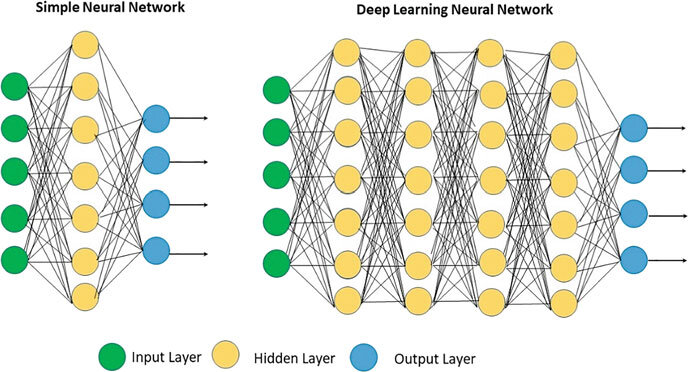
\includegraphics[width=0.8\textwidth]{imgs/neural_vs_deep.png}
\caption{Comparison between traditional neural networks (left) and deep learning architectures (right), illustrating the difference in complexity and hierarchical feature learning capabilities.}
\label{fig:neural_vs_deep}
\end{figure}

Deep learning architectures consist of multiple hidden layers, each containing many artificial neurons (nodes) that process information through weighted connections. Each neuron receives inputs, applies a weighted sum followed by an activation function, and passes the result to subsequent layers. This layered structure enables the network to learn increasingly complex and abstract representations, with early layers capturing low-level features and deeper layers combining these into high-level patterns. The depth of these networks allows them to model complex, non-linear relationships that are particularly valuable for complex temporal data such as battery wear patterns.

For this project, the deep learning approach was specifically chosen due to its superior ability to capture complex temporal patterns inherent in battery wear data and its capacity to handle the high-dimensional, sequential nature of battery health monitoring without requiring extensive domain-specific preprocessing or manual feature design. Deep learning excels in battery applications because it can automatically discover relevant features from raw sensor measurements (voltage, current, temperature) and learn the subtle, non-linear relationships between these measurements and battery health states. The hierarchical feature learning capability is particularly important for battery data, where wear patterns show across multiple time scales and involve complex interactions between chemical processes. Furthermore, deep learning architectures such as recurrent neural networks (RNNs), Long Short-Term Memory (LSTM) networks, and Transformers are specifically designed to handle sequential data, making them ideal for modeling the temporal dependencies present in battery operational data and predicting future health states based on historical patterns.


\vspace{1cm}

\textbf{Deep Learning Training Parameters and Optimization}

Understanding key training parameters is crucial for developing effective battery state estimation models. \textbf{Epochs} represent complete passes through the training dataset, where 50--500 epochs are typical for battery data, carefully balancing the risk of underfitting with too few iterations against overfitting with excessive training on temporal sequences. \textbf{Batch Size} determines the number of samples processed at the same time, where smaller batches (16--32) excel at capturing nonlinear patterns in battery behavior, while larger batches (128--256) provide more stable gradients but may struggle with the irregular nature of real-world battery data.

\textbf{Patience} in early stopping mechanisms defines how many epochs to wait without validation improvement before ending training, with values of 5--20 epochs proving effective at preventing overfitting while allowing models sufficient time to generalize across different battery systems and operational conditions. \textbf{Learning Rate} controls the size of parameter adjustments during training, requiring careful tuning for battery wear patterns: rates too high (>0.01) risk missing subtle wear signals, while rates too low (<0.0001) result in painfully slow convergence and potentially incomplete learning.

\textbf{Optimizers} play a critical role in training efficiency, with the Adam optimizer commonly chosen for its adaptive learning rate capabilities, while SGD with momentum provides more stable convergence but demands additional hyperparameter tuning specifically for battery applications. \textbf{Regularization} techniques, including L1/L2 regularization and dropout, become particularly important when working with limited battery datasets, especially when training data comes from only a few battery types or specific operational conditions.

\textbf{Loss Functions} must be carefully selected based on the specific task: MSE for regression problems like SoC and capacity prediction, MAE when robustness against outliers is most important, cross-entropy for classification tasks such as fault detection, and custom loss functions that can elegantly incorporate domain-specific knowledge about battery behavior. Finally, \textbf{Validation} strategies require special consideration in battery applications, where time-based splitting ensures models are tested on genuinely future data, and cross-validation procedures must account for the inherent temporal dependencies present in battery wear sequences.


\vspace{1cm}
\textbf{Battery Degradation and Capacity Fade}
\label{sec:degradation}

Battery wear refers to the gradual loss of a battery's ability to store and deliver energy, driven by chemical reactions, temperature changes, charge/discharge cycles, and aging. This wear shows as capacity fade, resulting in reduced device runtime or diminished electric vehicle driving range. The key mechanisms contributing to this wear include several interconnected processes. \textbf{Solid Electrolyte Interphase (SEI) Growth} occurs when a layer forms on the anode, consuming lithium ions and reducing capacity. This process is accelerated at high temperatures and currents, leading to an initial irreversible capacity loss of approximately 10\% during formation cycles. \textbf{Lithium Plating} represents another critical mechanism where, at low temperatures or high charge rates, lithium deposits on the anode, forming ``dead lithium'' that contributes to irreversible capacity loss and increases safety risks. \textbf{Particle Fracture} results from mechanical stress during cycling, causing cracks in electrode materials that reduce active material availability and make capacity decline worse. \textbf{Positive Electrode (PE) Decomposition} involves structural changes in the cathode, such as spinel/rock salt phase formation, which degrade performance and contribute to active material loss. Finally, \textbf{Impedance Increase} shows as rising interfacial resistance, mainly at the positive electrode, which limits efficient charge transfer and indirectly reduces usable capacity. After 800 cycles, electrode resistance can increase tenfold, significantly impacting battery performance.

\vspace{1cm}
\textbf{Capacity Fade}
The \cite{zhang_studies_2000} paper studies and explains very well the capacity fade refers to the progressive decline in a lithium-ion battery’s ability to store energy, manifesting as reduced device runtime or diminished electric vehicle driving range. This phenomenon is driven by several key mechanisms:

Studies report capacity losses ranging from 12.4\% to 32\% after 500--800 cycles, corresponding to an average loss of 0.025--0.05\% per cycle~\cite{zhang_studies_2000}.

\textbf{Internal Resistance Degradation in Lithium-Ion Batteries}

As lithium-ion batteries age, their internal resistance increases, badly affecting power delivery, charging efficiency, and thermal management. This wear is particularly noticeable during calendar ageing, as detailed in the study by \cite{stroe_degradation_2018} on LFP/C-based batteries. The primary mechanisms contributing to this increase involve several interconnected processes. \textbf{Solid Electrolyte Interface (SEI) Growth} is characterized by the thickening of the SEI layer on the graphite anode over time, reducing Li$^+$ ion permeability. This growth follows a power law dependence (approximately $t^{0.8}$) and is accelerated at high temperatures and high state-of-charge (SOC) levels, leading to increased resistance and contact loss within the anode. \textbf{Lithium Plating} involves the deposition of metallic lithium on the anode, which clogs electrode pores, blocking ion transport and elevating resistance, particularly under high SOC conditions. \textbf{Cathode Structural Degradation} occurs at the LFP cathode, where binder decomposition, oxidation of conductive agents, and corrosion of current collectors reduce inter-particle conductivity, contributing to resistance increase, especially at elevated temperatures. Also, \textbf{Electrolyte Decomposition} produces decomposition products that form resistive surface layers on both electrodes, further increasing internal resistance, with effects amplified at high temperatures and SOC levels.

The study shows that internal resistance increases nonlinearly with storage time, with exponential acceleration due to higher storage temperatures (e.g., 55°C) and SOC levels (e.g., 90\%). For instance, after 20 years at 25°C and 50\% SOC, resistance may rise by approximately 71\%, doubling at 100\% SOC. This increased resistance results in slower charging, reduced power output, and accelerated wear due to enhanced heat generation, impacting battery performance and lifespan.

\textbf{Battery Health Monitoring}

Battery health monitoring is critical for ensuring reliability, safety, and longevity of battery systems. Monitoring involves checking key parameters such as the state of charge and the state of health (SoH), which provide essential insights into battery performance and remaining operational capacity.

\textbf{Technical Challenges}
The technical challenges in monitoring battery health come from the complex nature of battery systems and the difficulties in accurately estimating SOC and SOH.

\vspace{1cm}
\textbf{Complexity of Battery Chemistry}

Batteries, particularly lithium-ion batteries, have complex internal chemistries that are difficult to model and monitor.
Factors such as temperature, charge-discharge rates, and depth of discharge influence wear, making accurate SOH estimation challenging. 
The nonlinear and complex wear processes vary with usage conditions, environmental factors, and battery design, complicating predictive modeling.

\vspace{1cm}
\textbf{Measurement Difficulties}

Measuring individual battery parameters, such as internal resistance, temperature, and voltage, is technically challenging, especially in real-time applications. 
This requires precise sensors and sophisticated equipment, which may not be possible in real-world scenarios. 
For instance, accurately measuring internal resistance or temperature in a moving vehicle is far more complex than in a controlled lab environment.

\vspace{1cm}
\textbf{Modeling and Estimation}

\textbf{rever isto !!!} \\
Developing accurate models for SOH estimation is complex. 
Chemical models, which simulate battery behavior based on physical and chemical principles, require extensive computational resources and detailed parameter inputs (e.g., electrolyte properties, reaction rates). 
Semi-empirical models often oversimplify chemical processes, reducing their effectiveness under extreme conditions. Equivalent circuit models (ECMs) may lack precision during high-rate charging/discharging or extreme temperatures due to their simplified nature.

\vspace{1cm}
\textbf{Limitations of Data-Driven Methods}

Data-driven approaches, such as machine learning techniques (e.g. Support Vector Regression, Gaussian Process Regression, Artificial Neural Networks), rely on large, high-quality datasets, which can be difficult to obtain. 
These methods also lack physical understanding, making it difficult to understand their predictions. 
Also, issues like overfitting and high computational demands pose challenges for real-time applications.

\vspace{1cm}
\textbf{Complexity of Hybrid Methods}

Hybrid approaches, which combine model-based and data-driven methods, can improve accuracy but increase system complexity and computational costs. 
Understanding errors in these systems remains a challenge, requiring further research to enhance transparency and efficiency.

\vspace{1cm}
\textbf{Laboratory vs Real World Conditions}

There is a significant difference between laboratory-simulated conditions and actual operational environments. 
Laboratory settings often use sophisticated equipment that is not available in real-world applications, limiting the applicability of monitoring methods. For example, real-world conditions like varying temperatures or road vibrations are difficult to replicate in a lab, affecting SOH estimation accuracy.

\vspace{1cm}
\textbf{Real-Time Monitoring}

Getting real-time, reliable SOH monitoring is crucial for safety-critical applications but is technically demanding. 
Battery management systems (BMS) must balance accuracy with computational efficiency to provide timely insights without overloading system resources.

\vspace{1cm}
\textbf{Environmental Factors}

Batteries are sensitive to environmental conditions such as temperature, humidity, and vibration. 
Monitoring systems must account for these factors, which can significantly impact battery health and performance. 
For example, high temperatures can accelerate battery wear, while low temperatures may reduce capacity, complicating health estimation.

\vspace{1cm}
\textbf{Cost of Monitoring Systems}

Setting up sophisticated battery health monitoring systems can be expensive, both in terms of initial setup and ongoing maintenance. 
This includes the cost of sensors, data storage, and computational infrastructure, which can be too expensive for smaller organizations or applications.

\vspace{1cm}
\textbf{Data and Computational Costs}

AI and data-driven methods require significant computational resources and high-quality data, which can be costly to acquire and process. 
The high demand for data and computing power presents challenges, particularly for real-time monitoring applications and edge devices.

%\section{Supporting Technologies}
%Sensor technologies for battery data collection
%Data acquisition systems and protocols
%Computing platforms/hardware used

%\section{Methodogical Background}
%Signal processing techniques for battery data
%Feature extraction methods
%Relevant machine learning algorithms (classification, regression, etc.)
%Evaluation metrics for health monitoring systems

%\section{Related Frameworks}
%Software libraries and tools used in implementation
%Data management approaches
%Visualization techniques

\section{Supporting Technologies}

This section describes the complete suite of software tools and platforms that helped the research and development process, including analytical frameworks, optimization tools, and development environments.

\textbf{Optuna}
\label{subsec:optuna}
Optuna is an open-source hyparameter tuning framework used to search for the best parameters in machine learning models~\cite{akiba_optuna_2019}. It uses algorithms like Tree-structured Parzen Estimator (TPE) to systematically explore parameter spaces, supporting parallel and distributed optimization. In this work, Optuna was used to automate the tuning process, improving model performance by identifying optimal parameter configurations with reduced manual effort.

\textbf{Weights and Biases (WandB)}
\label{subsec:wandb}
Weights \& Biases (WandB) is a machine learning platform designed for experiment tracking and display~\cite{noauthor_weights_nodate}. It enables real-time logging and monitoring of training metrics, parameters, and model outputs. In this study, WandB was used to keep track of training processes and display losses, providing interactive dashboards to analyze experiments.

\textbf{PlotJuggler}
PlotJuggler is an open-source time series display tool designed for fast, easy-to-use, and extensible data analysis~\cite{faconti_facontidavideplotjuggler_2025}. It features a user-friendly drag-and-drop interface, enabling efficient display of large datasets. In this work, PlotJuggler was highly effective for exploring and analyzing data within datasets, allowing for the display of time series, identification of patterns. Its a valuable tool for detailed data inspection and analysis.

\textbf{Orange Data Mining}
Orange Data Mining is an open-source data display and analysis platform designed for exploratory data analysis and machine learning workflows~\cite{noauthor_biolaborange3_nodate}. It provides a visual programming interface with drag-and-drop widgets that enable users to build data analysis pipelines without extensive coding. Orange offers complete tools for data preprocessing, feature selection, correlation analysis, and outlier detection through interactive displays and statistical methods. In this work, Orange was important for exploring correlations within battery datasets and identifying outliers that could potentially skew model performance.

\textbf{Git Version Control}
Git is a distributed version control system designed to handle projects of all sizes with speed and efficiency~\cite{noauthor_git_nodate}. It tracks changes in source code and files during software development,maintaining a complete history of modifications. Git provides features such as branching, merging. In this work, Git was used to ensure version control throughout the research process, maintaining a complete history of code changes, experimental iterations, and documentation updates. All project files, including machine learning models, data processing scripts, and analysis, were committed and pushed to GitHub repositories.

\textbf{PyTorch}
PyTorch is an open-source machine learning framework developed by Facebook's AI Research lab, designed for deep learning applications with a 
focus on flexibility and ease of use~\cite{ansel_pytorch_2024}. It provides dynamic computational graphs, 
allowing for easy model development and debugging through its eager execution model. PyTorch features 
automatic differentiation capabilities through its autograd system, enabling efficient gradient computation 
for backpropagation in neural networks. The framework supports GPU acceleration through CUDA, making it suitable
for training large-scale models efficiently. 

PyTorch was specifically chosen over TensorFlow for this project due to several key advantages that align with the research requirements. \textbf{Research-oriented design} provides greater flexibility for implementing novel architectures and custom loss functions specific to battery wear modeling, whereas TensorFlow's static graph approach can be more restrictive for experimental work. Also, \textbf{superior community support} in the academic research community and \textbf{extensive documentation}.

In this work, PyTorch served as the primary framework for developing and training deep learning models for battery health monitoring applications. PyTorch smoothly integrates with other tools in the machine learning pipeline, such as Optuna (see Section~\ref{subsec:optuna}) for automated parameter tuning and WandB (see Section~\ref{subsec:wandb}) for comprehensive experiment tracking, creating a cohesive development environment that supports reproducible research workflows.

\textbf{Conda Environments}
Conda is an open-source package management and environment management system that simplifies the installation, running, and updating of packages and 
their dependencies~\cite{conda_contributors_conda_2025}. It creates isolated environments where different versions of Python, libraries, 
and dependencies can coexist without conflicts, making it particularly valuable for this projects. This approach ensured that version conflicts between packages were avoided, enabled smooth collaboration across different 
development machines, and guaranteed that the exact software environment could be recreated for reproducibility.

